\chapter{Atomic Cross Sections}\label{app:cross_sections}
\newpage
\section{Hydrogen-Hydrogen Interactions}
\subsection{Charge Exchange: $H^+ + H(n) \rightarrow H(m) + H^+$}
\subsubsection{References}
\begin{itemize}
    \item ADAS\cite{adas}
    \item Equation 44 and Table 9 in Janev\cite{janev2003collision}
\end{itemize}
\subsubsection{Hydrogen Charge Exchange Cross Sections}
\begin{figure}[h!]%
    \centering
    \subfigure[][]{%
        \label{fig:H_H_CX_1}
        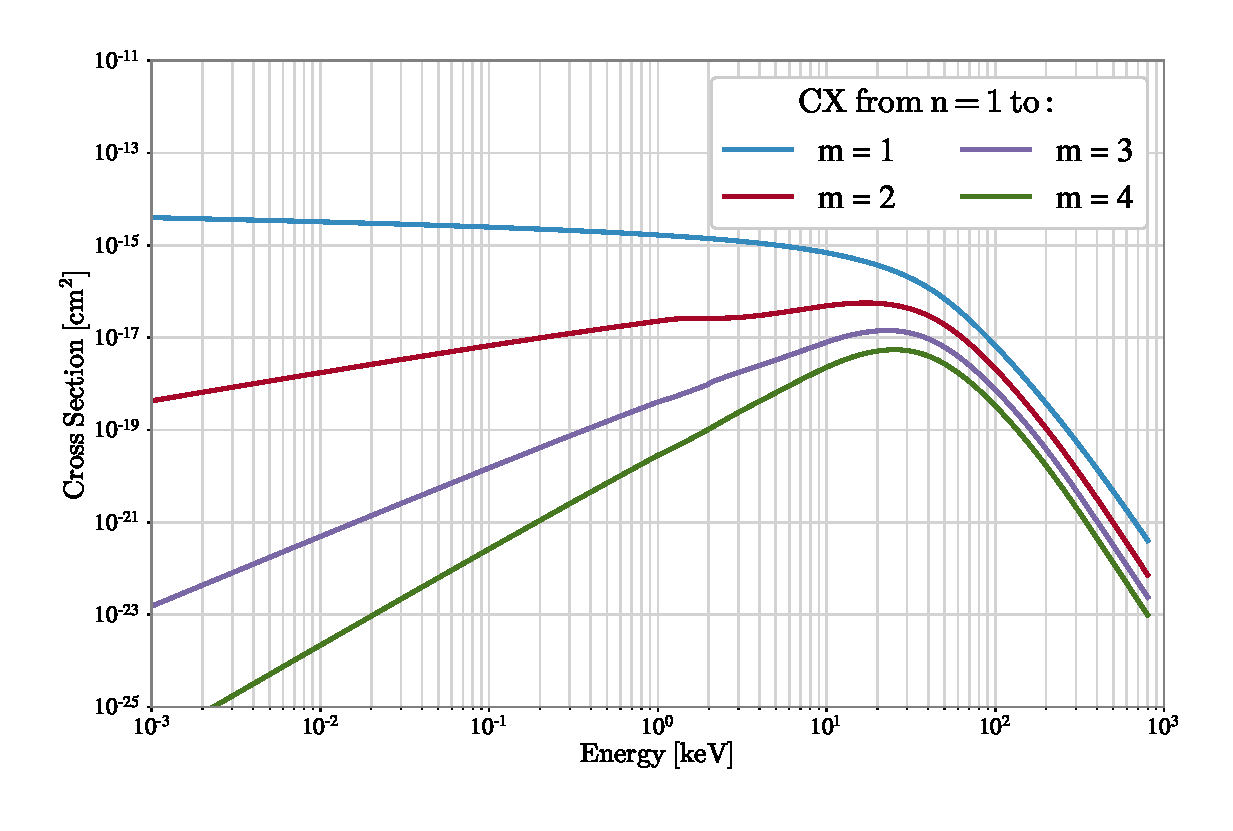
\includegraphics[height=1.9in]{tables/H_H_cx_1_m.eps}}
    \hspace{8pt}
    \subfigure[][]{
        \label{fig:H_H_CX_2}
        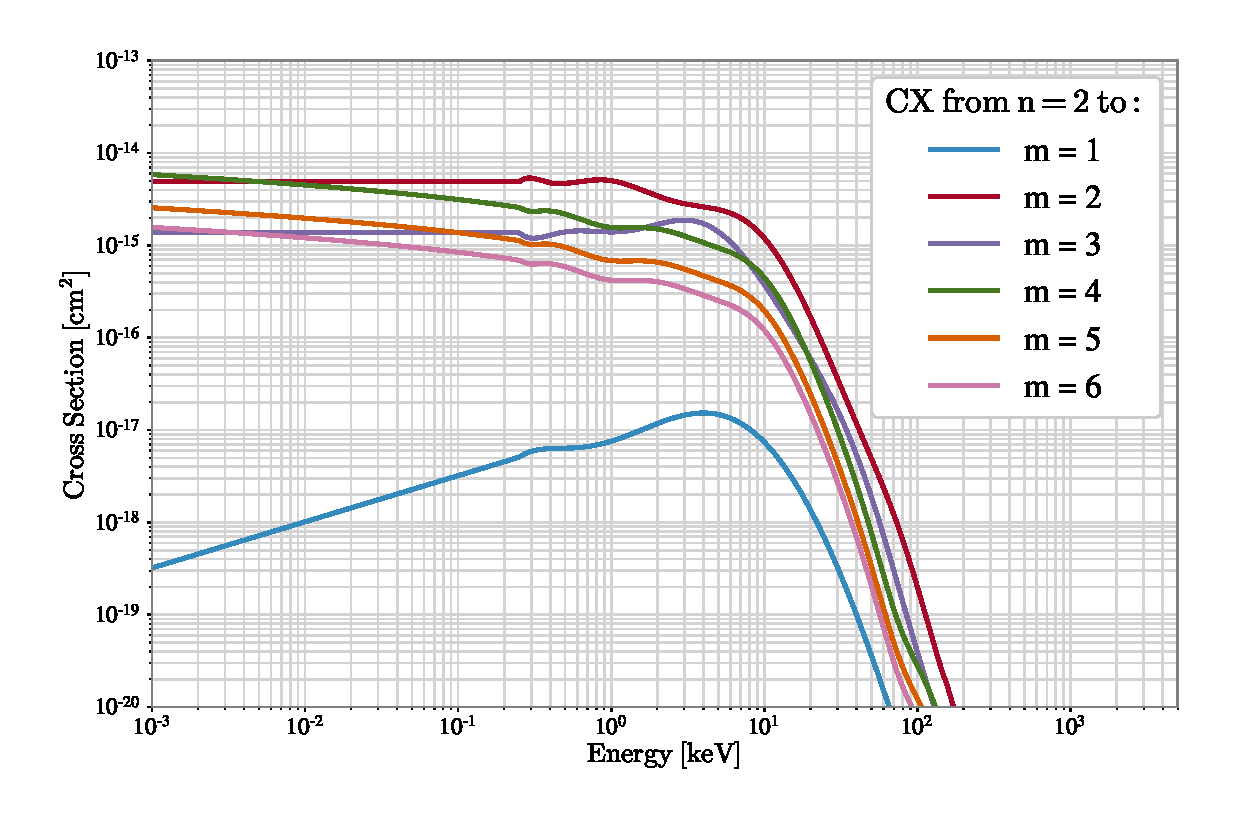
\includegraphics[height=1.9in]{tables/H_H_cx_2_m.eps}} \\
    \subfigure[][]{
        \label{fig:H_H_CX_3}
        \includegraphics[height=1.9in]{tables/H_H_cx_3_m.eps}}
    \hspace{8pt}
    \subfigure[][]{
        \label{fig:H_H_CX_4}
        \includegraphics[height=1.9in]{tables/H_H_cx_4_m.eps}}
    \caption{Hydrogen-Hydrogen charge exchange cross sections:
        \subref{fig:H_H_CX_1} charge exchange from the $n=1$ level;
        \subref{fig:H_H_CX_2} charge exchange from the $n=2$ level;
        \subref{fig:H_H_CX_3} charge exchange from the $n=3$ level; and,
        \subref{fig:H_H_CX_4} charge exchange from the $n=4$ level.}
    \label{fig:H_H_CX}
\end{figure}
\newpage

\subsection{Excitation: $H^+ + H(n) \rightarrow H^+ + H(m), m > n$}
\subsubsection{References}
\begin{itemize}
    \item Equation 29.b and Table 4 in Janev\cite{janev2003collision} for $n=1$ and $m=2$
    \item Equation 30 and Table 5 in Janev\cite{janev2003collision} for $n=1$ and $m=3-6$
    \item Equation 31 and Table 5 in Janev\cite{janev2003collision} for $n=1$ and $m>6$
    \item Equation 32 and Table 6 in Janev\cite{janev2003collision} for $n=2$ and $m\le5$
    \item Equation 33 and Table 6 in Janev\cite{janev2003collision} for $n=2$ and $m=6-10$
    \item Equation 34 and Table 6 in Janev\cite{janev2003collision} for $n=2$ and $m>10$
    \item Equation 35 and Table 7 in Janev\cite{janev2003collision} for $n=3$ and $m\le6$
    \item Equation 36 and Table 7 in Janev\cite{janev2003collision} for $n=3$ and $m7-106$
    \item Equation 37 and Table 7 in Janev\cite{janev2003collision} for $n=3$ and $m>10$
    \item Equation 38-39 in Janev\cite{janev2003collision} for $n>3$ and $m>4$
\end{itemize}
\newpage
\subsubsection{Hydrogen Excitation Cross Sections}
\begin{figure}[h!]%
    \centering
    \subfigure[][]{%
        \label{fig:H_H_EX_1}
        \includegraphics[height=2in]{tables/H_H_excit_1_m.eps}}
    \hspace{8pt}
    \subfigure[][]{
        \label{fig:H_H_EX_2}
        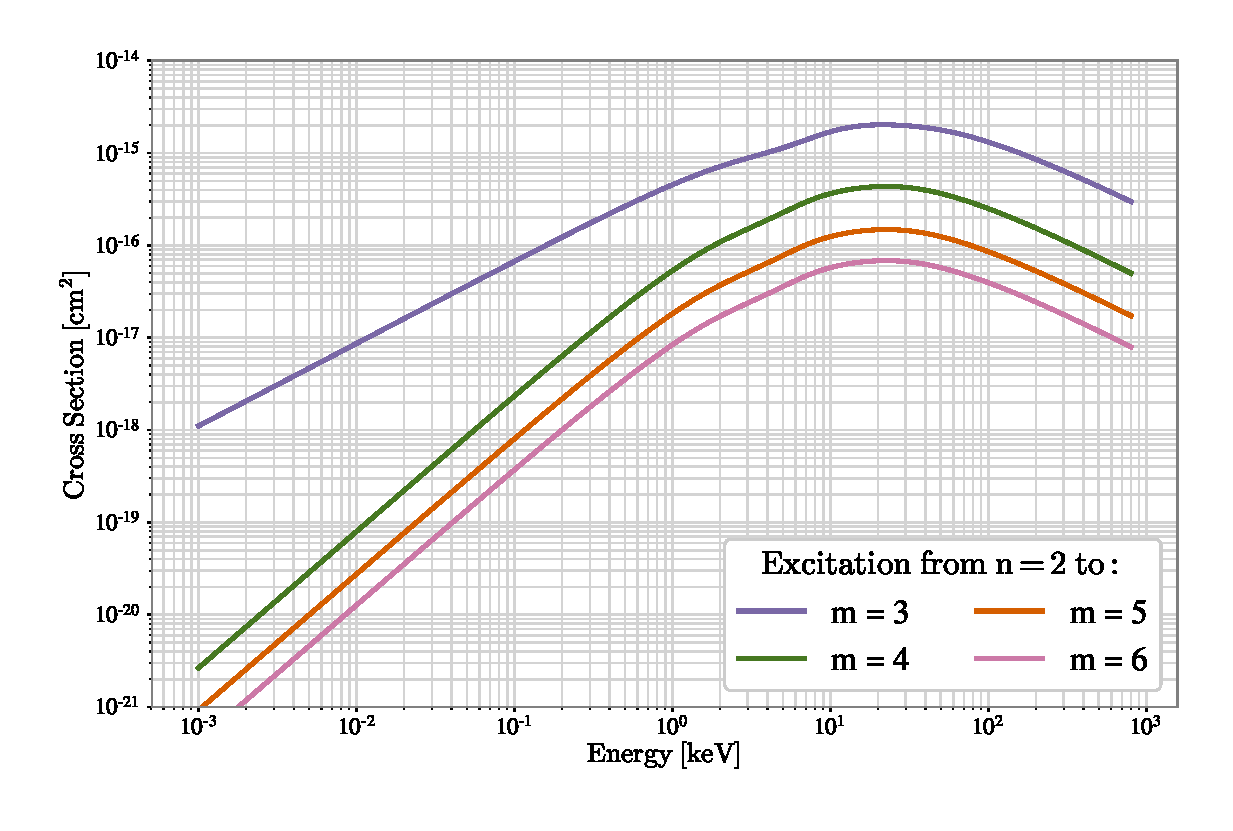
\includegraphics[height=2in]{tables/H_H_excit_2_m.eps}} \\
    \subfigure[][]{
        \label{fig:H_H_EX_3}
        \includegraphics[height=2in]{tables/H_H_excit_3_m.eps}}
    \hspace{8pt}
    \subfigure[][]{
        \label{fig:H_H_EX_4}
        \includegraphics[height=2in]{tables/H_H_excit_4_m.eps}}
    \caption{Hydrogen-Hydrogen excitation cross sections:
        \subref{fig:H_H_EX_1} excitation from the $n=1$ level;
        \subref{fig:H_H_EX_2} excitation from the $n=2$ level;
        \subref{fig:H_H_EX_3} excitation from the $n=3$ level; and,
        \subref{fig:H_H_EX_4} excitation from the $n=4$ level.}
    \label{fig:H_H_EX}
\end{figure}
\newpage
\subsection{Ionization: $H^+ + H(n) \rightarrow H^+ + H^+ + e$}
\subsubsection{References}
\begin{itemize}
    \item Equation 40 and Table 8 in Janev\cite{janev2003collision} for $n=1$
    \item Equation 5 and Table 1 in O'Mullane\cite{omullane2009review} for $n\ge2$
\end{itemize}
\subsubsection{Hydrogen Ionization Cross Sections}
\begin{figure}[h!]
    \centering
    \includegraphics[width=10cm]{figures/tables/H_H_ioniz.eps}
    \caption{Hydrogen-Hydrogen ionization cross sections from different $n$ levels.}
    \label{fig:H_H_ioniz}
\end{figure}
\newpage

\section{Hydrogen-Electron Interactions}
\subsection{Excitation: $e + H(n) \rightarrow e + H(m), m > n$}
\subsubsection{References}
\begin{itemize}
    \item Equation 5 and Table 2 in Janev\cite{janev2003collision}
    \item Equation 6-7 in Janev\cite{janev2003collision}
    \item Section 2.1.1 B in Janev\cite{janev2003collision}
\end{itemize}
\subsubsection{Electron Excitation Cross Sections}
\begin{figure}[h!]%
    \centering
    \subfigure[][]{%
        \label{fig:H_E_EX_1}
        \includegraphics[height=1.7in]{tables/H_e_excit_1_m.eps}}
    \hspace{8pt}
    \subfigure[][]{
        \label{fig:H_E_EX_2}
        \includegraphics[height=1.7in]{tables/H_e_excit_2_m.eps}} \\
    \subfigure[][]{
        \label{fig:H_E_EX_3}
        \includegraphics[height=1.7in]{tables/H_e_excit_3_m.eps}}
    \hspace{8pt}
    \subfigure[][]{
        \label{fig:H_E_EX_4}
        \includegraphics[height=1.7in]{tables/H_e_excit_4_m.eps}}
    \caption{Hydrogen-Electron excitation cross sections:
        \subref{fig:H_E_EX_1} excitation from the $n=1$ level;
        \subref{fig:H_E_EX_2} excitation from the $n=2$ level;
        \subref{fig:H_E_EX_3} excitation from the $n=3$ level; and,
        \subref{fig:H_E_EX_4} excitation from the $n=4$ level.}
    \label{fig:H_E_EX}
\end{figure}
\newpage

\subsection{Ionization: $e + H(n) \rightarrow e + H^+ + e$}
\subsubsection{References}
\begin{itemize}
    \item Equation 14 and Table 3 in Janev\cite{janev2003collision}
    \item Equation 15-16 in Janev\cite{janev2003collision}
\end{itemize}
\subsubsection{Electron Ionization Cross Sections}
\begin{figure}[h!]
    \centering
    \includegraphics[width=10cm]{figures/tables/H_e_ioniz.eps}
    \caption{Hydrogen-Electron ionization cross sections from different $n$ levels.}
    \label{fig:H_E_ioniz}
\end{figure}
\newpage

\section{Hydrogen-Impurity Interactions}
\subsection{Charge Exchange: $A^{q} + H(n) \rightarrow A^{(q-1)+} + H^+$}
\subsubsection{References}
\begin{itemize}
    \item ADAS\cite{adas}
    \item $B^{5+}$: Page 166 in Janev1993\cite{janev1993cross} for $n=1$
    \item $C^{6+}$: Page 168 in Janev1993\cite{janev1993cross} for $n=1$
    \item $A^{q+}$: Page 174 in Janev1993\cite{janev1993cross} for $n>1,q>3$
\end{itemize}
\subsubsection{Carbon Charge Exchange Cross Sections}
\begin{figure}[h!]
    \centering
    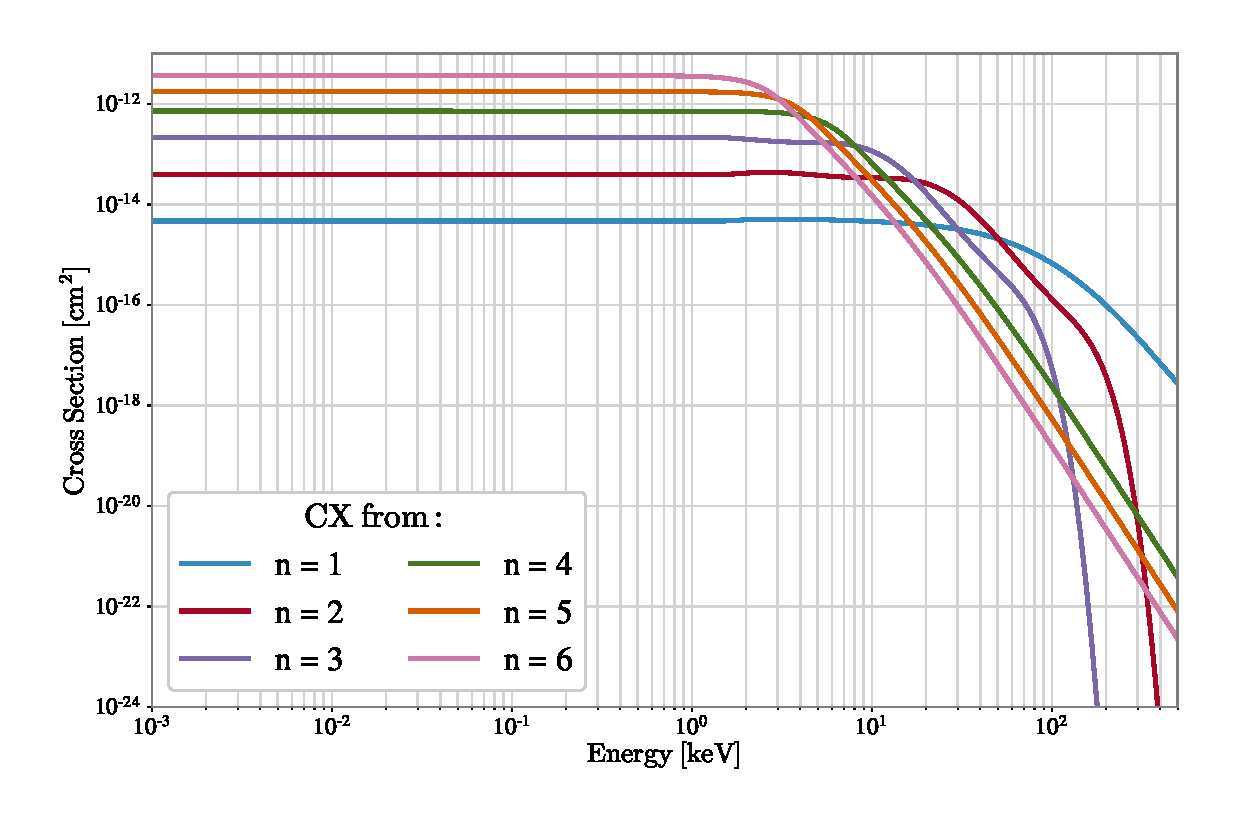
\includegraphics[width=10cm]{figures/tables/H_C6_cx.eps}
    \caption{Hydrogen-Carbon charge exchange cross sections from different $n$ levels.}
    \label{fig:H_C6_CX}
\end{figure}
\newpage

\subsection{Excitation: $C^{6+} + H(n) \rightarrow C^{6+} + H(m), m > n$}
\subsubsection{References}
\begin{itemize}
    \item $A^{q+}$: Page 132 in Janev1993\cite{janev1993cross} for $n=1,m=2,q>4$
    \item $A^{q+}$: Page 134 in Janev1993\cite{janev1993cross} for $n=1,m=3-4,q>3$
    \item $A^{q+}$: Page 136 in Janev1993\cite{janev1993cross} for $n=1,m>4,q>4$
    \item $A^{q+}$: Page 138 in Janev1993\cite{janev1993cross} for $n=2,m=3-5,q>3$
    \item $A^{q+}$: Page 140 in Janev1993\cite{janev1993cross} for $n=2,m>5,q>3$
    \item $A^{q+}$: Page 142 in Janev1993\cite{janev1993cross} for $n=3,m=4-6,q>3$
    \item $A^{q+}$: Page 144 in Janev1993\cite{janev1993cross} for $n=3,m>6,q>3$
    \item $A^{q+}$: Page 146 in Janev1993\cite{janev1993cross} for $n>3,m>n,q>3$
\end{itemize}
\newpage
\subsubsection{Carbon Excitation Cross Sections}
\begin{figure}[h!]%
    \centering
    \subfigure[][]{%
        \label{fig:H_C6_EX_1}
        \includegraphics[height=2in]{tables/H_C6_excit_1_m.eps}}
    \hspace{8pt}
    \subfigure[][]{
        \label{fig:H_C6_EX_2}
        \includegraphics[height=2in]{tables/H_C6_excit_2_m.eps}} \\
    \subfigure[][]{
        \label{fig:H_C6_EX_3}
        \includegraphics[height=2in]{tables/H_C6_excit_3_m.eps}}
    \hspace{8pt}
    \subfigure[][]{
        \label{fig:H_C6_EX_4}
        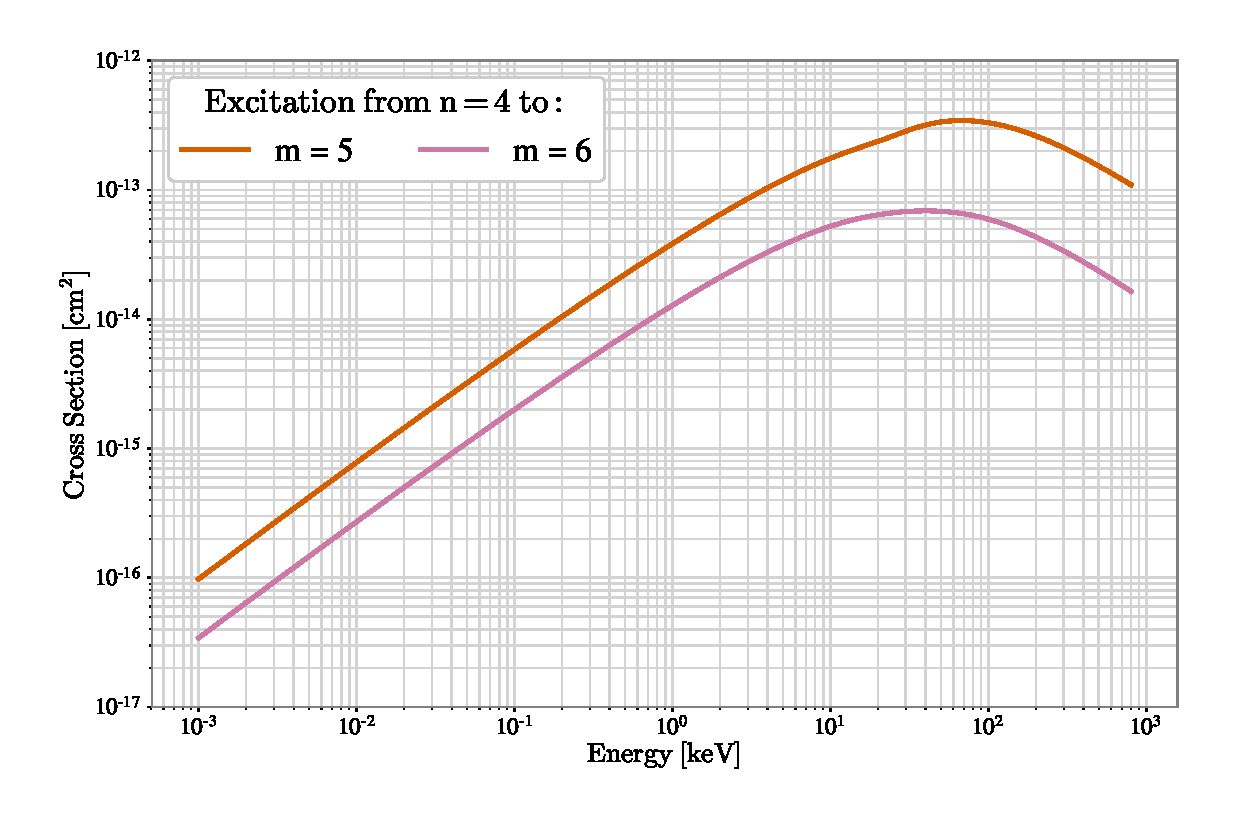
\includegraphics[height=2in]{tables/H_C6_excit_4_m.eps}}
    \caption{Hydrogen-Carbon excitation cross sections:
        \subref{fig:H_C6_EX_1} excitation from the $n=1$ level;
        \subref{fig:H_C6_EX_2} excitation from the $n=2$ level;
        \subref{fig:H_C6_EX_3} excitation from the $n=3$ level; and,
        \subref{fig:H_C6_EX_4} excitation from the $n=4$ level.}
    \label{fig:H_C6_EX}
\end{figure}
\newpage

\subsection{Ionization: $A^{q+} + H(n) \rightarrow A^{q+} + H^+ + e$}
\subsubsection{References}
\begin{itemize}
    \item ADAS\cite{adas}
    \item $B^{5+}$: Page 152 in Janev1993\cite{janev1993cross} for $n=1$
    \item $C^{6+}$: Page 154 in Janev1993\cite{janev1993cross} for $n=1$
    \item $A^{q+}$: Page 160 in Janev1993\cite{janev1993cross} for $n>1,q>3$
\end{itemize}
\subsubsection{Carbon Ionization Cross Sections}
\begin{figure}[h!]
    \centering
    \includegraphics[width=10cm]{figures/tables/H_C6_ioniz.eps}
    \caption{Hydrogen-Carbon ionization cross sections from different $n$ levels.}
    \label{fig:H_C6_ioniz}
\end{figure}